% Creado por Johautt Hernández
% Licenciado bajo la normativa del archivo license del directorio raíz

\documentclass[12pt, twoside, openright]{book}

% --- 1. Paquetes Esenciales (Idioma y Codificación) ---
\usepackage[utf8]{inputenc} % Codifica texto en UTF8
\usepackage[T1]{fontenc}    % Para las fuentes
\usepackage[spanish]{babel} % Configura el idioma a español
\usepackage{csquotes}       % Necesario para biblatex/babel
\usepackage{lipsum}         % Genera texto de ejemplo (tipo Lorem Ipsum)


% --- 2. PAQUETES DE FORMATO UNEFA/TEG ---
\usepackage{geometry}  % A menudo necesario para un mejor manejo de márgenes en diagramas anchos
\usepackage{setspace}  % Para el interlineado vertical (1.0, 1.5 o 2.0)
\usepackage{fancyhdr}  % Para el manejo de las cabeceras y piés de página
\usepackage{graphicx}  % Para insertar
\usepackage{ragged2e}  % Para la justificación del texto
\usepackage{pgfgantt}  % Para el manejo de diagramas de Gantt
\usepackage{pdflscape} % Permite rotar una sola página, útil para figuras grandes com el diagrama de Gantt
\usepackage{xcolor}    % Para colores en el diagrama
\usepackage{emptypage} % Para que las hojas insertadas por \cleardoublepage tengan estilo vacío
\usepackage{amsmath, amsthm, amssymb} % Para el uso de fórmulas matemáticas.

% --- 3. Carga de Datos y Variables (con \input) ---
% Aquí se cargan \title, \author, y los \newcommand para la portada/aprobación.
% -------------------------------------------------------------
% METADATOS
% -------------------------------------------------------------

% --- DATOS DE LA PORTADA ---
\newcommand{\unefaNucleo}{NÚCLEO ARAGUA - SEDE MARACAY}
% UNIDAD (DESCOMENTAR SI EXISTE)
%\newcommand{\unefaUnidad}{E.A.D. DE INVESTIGACIÓN}
\newcommand{\carrera}{Escribir Carrera Aquí}
\newcommand{\tipoTrabajo}{Trabajo Especial de Grado}
\newcommand{\datosTitulo}{ANÁLISIS DE FALLAS EN SISTEMAS EMBEBIDOS UTILIZANDO REDES NEURONALES}
\newcommand{\tituloCorto}{COLOCAR ENCABEZADO CORTO AQUÍ}

% --- DATOS DEL AUTOR(ES) Y TUTOR ---
% TUTOR
\newcommand{\datosTutorNombre}{Federico Pinto}
\newcommand{\datosTutorCI}{V-1.234.567}
\newcommand{\datosTutorTitulo}{Ing.}
% PRIMER AUTOR
\newcommand{\datosAutorNombre}{Pepito Pérez}
\newcommand{\datosAutorCI}{V-9.876.543}
% SEGUNDO AUTOR (DESCOMENTAR SI EXISTE)
%\newcommand{\datosSegAutorNombre}{Petra Gómez}
\newcommand{\datosSegAutorCI}{V-10.987.654}
% TÍTULO DE AMBOS AUTORES
\newcommand{\datosAutoresTitulo}{Br.}

% --- DATOS DE LUGAR Y FECHA ---
% CIUDAD PRESENTACIÓN
\newcommand{\cuidadPresentacion}{Maracay}
% ESTADO PRESENTACIÓN
\newcommand{\estadoPresentacion}{Aragua}

% 1. El día de presentación (ej. 28)
\newcommand{\diaPresentacion}{28}

% 2. El MES de presentación se define como un NÚMERO (1=Enero, 9=Septiembre, 11=Noviembre)
\newcommand{\mesNumPresentacion}{11} % <--- ¡Define el mes como un número!

% 3. El año (ej. 2025)
\newcommand{\anoPresentacion}{2025}

% --- METADATOS ESTÁNDAR (Usan la variable) ---
\date{\fechaPresentacion}
\author{\datosAutorNombre}
\title{\datosTitulo}
% --- LÓGICA DE LA ETIQUETA ---
% 1. Definimos una macro para el texto de la etiqueta de Autor
% 2. Verificamos si el segundo autor está definido.
% 3. Si está definido, la etiqueta es "Autores:", si no, es "Autor(a):"
\ifdefined\datosSegAutorNombre
    \newcommand{\etiquetaAutor}{\textbf{Autores:}}
\else
    \newcommand{\etiquetaAutor}{\textbf{Autor(a):}}
\fi

% Redefinimos lugarPresentacion
\newcommand{\lugarPresentacion}{\cuidadPresentacion, Edo. \estadoPresentacion}

% Macro para convertir número de mes (1-12) a formato numérico con relleno (01-12).
% El comando \ifcase es nativo de TeX. El #1 representa el argumento (el número de mes).
\newcommand{\MesANumerico}[1]{%
    \ifcase#1\relax
        % El caso 0 queda vacío.
    \or 01% 1: Enero
    \or 02% 2: Febrero
    \or 03% 3: Marzo
    \or 04% 4: Abril
    \or 05% 5: Mayo
    \or 06% 6: Junio
    \or 07% 7: Julio
    \or 08% 8: Agosto
    \or 09% 9: Septiembre
    \or 10% 10: Octubre
    \or 11% 11: Noviembre
    \or 12% 12: Diciembre
    \fi
}

% También puedes definir el nombre del mes para la portada (Noviembre, 2025)
\newcommand{\MesANombre}[1]{%
    \ifcase#1\relax
    \or Enero% 1
    \or Febrero% 2
    \or Marzo% 3
    \or Abril% 4
    \or Mayo% 5
    \or Junio% 6
    \or Julio% 7
    \or Agosto% 8
    \or Septiembre% 9
    \or Octubre% 10
    \or Noviembre% 11
    \or Diciembre% 12
    \fi
}

% Redefinimos fechaPresentacion
\newcommand{\fechaPresentacion}{\MesANombre{\mesNumPresentacion}, \anoPresentacion}

% --- 4. CONFIGURACIÓN DEL FORMATO (UNEFA/TEG) ---

% 4.1. CONFIGURACIÓN DE MÁRGENES Y PAPEL
\geometry{
    letterpaper,
    top=3.0cm,
    bottom=3.0cm,
    right=3.0cm,
    left=4.0cm,
    includeheadfoot
}

% 4.2. ESPACIADO Y SANGRIAS
\doublespacing 
\setlength{\parindent}{1.27cm} % Sangría de 1.27 cm (0.5 pulgadas)

% CORRECCIÓN DE ENCABEZADO. TODO: buscar la manera de hacer innecesario esto
\setlength{\headheight}{14.61858pt} 
\addtolength{\topmargin}{-2.61858pt} 

% Configuración del encabezado (Running Head)
\pagestyle{fancy}
\fancyhead{} 
\fancyfoot{} 
\fancyhead[LE]{\nouppercase{\tituloCorto}}
\fancyhead[RO]{\nouppercase{\tituloCorto}}
\fancyhead[R]{\thepage} 

% --- 5. CITA LARGA (Bloque separado - Requisito UNEFA/TEG) ---
\renewcommand{\mkblockquote}[4]{%
  \singlespacing%
  \setattribute{block}{indent}{#2}%
  \setattribute{block}{label}{#3}%
  \setattribute{block}{postlabel}{#4}%
  \blx@begindlblock%
  #1%
  \blx@enddlblock%
}

% --- 6. CONFIGURACIÓN DE REFERENCIAS (¡ORDEN CORREGIDO AQUÍ!) ---
\usepackage[style=apa, sortcites=true, backend=biber]{biblatex} % 1. CARGAR EL PAQUETE
\addbibresource{referencias.bib}                            % 2. LUEGO AGREGAR EL ARCHIVO

% --- 7. ACTIVACIÓN DE HIPERVÍNCULOS (DEBE SER EL ÚLTIMO) ---
\usepackage[
    hidelinks,
    bookmarksnumbered=true,
    bookmarksopen=false,
]{hyperref}




\begin{document}
% =================================================================
% 1. PARTES PRELIMINARES (\frontmatter)
% Numera en romanos (i, ii, iii, ...)
% La numeración NO es visible hasta que se llama a \maketitle
% =================================================================
\frontmatter

% Portada y Contraportada (UNEFA Núcleo Anzoátegui separa estas páginas)
\thispagestyle{empty} % Asegura que no haya números de página ni encabezados en la portada.


% =========================================================
% 1. MEMBRETE INSTITUCIONAL (LOGO Y TEXTO OFICIAL)
% =========================================================
\begin{minipage}{0.5cm}
    \centering
    
\includegraphics[width=0.5cm,trim= 3cm 1cm 0.7cm 1cm]{imgs/logo_unefa.png}
\end{minipage}
\hfill
\begin{minipage}{13.5cm}
    \begin{singlespace}
        \centering
        \textbf{REPÚBLICA BOLIVARIANA DE VENEZUELA}\\
        \textbf{MINISTERIO DEL PODER POPULAR PARA LA DEFENSA}\\
        \textbf{UNIVERSIDAD NACIONAL EXPERIMENTAL POLITÉCNICA}
        \textbf{DE LA FUERZA ARMADA NACIONAL BOLIVARIANA}\\
        \textbf{\unefaNucleo}\\ % Extraído de datos.tex
        % =========================================================
        % 2. UNIDAD Y CARRERA
        % =========================================================
        \ifdefined\unefaUnidad
            \textbf{\unefaUnidad}\\ % Extraído de datos.tex
        \fi
        \textbf{CARRERA: \MakeUppercase{\carrera}} % Extraído de datos.tex
    \end{singlespace}
\end{minipage}

% ESPACIO FLEXIBLE
\vfill

\large
\begin{center}

    % =========================================================
    % 3. TÍTULO DEL TRABAJO
    % =========================================================
    \begin{singlespace}
        \textbf{\MakeUppercase{\datosTitulo}} % Usa la variable de texto
    \end{singlespace}

    % ESPACIO FLEXIBLE
    \vfill

    \normalsize

    % =========================================================
    % 5. TUTOR Y AUTOR/AUTORES (Sección de Firmas)
    % =========================================================

    % Columna izquierda - Tutor
    \begin{minipage}[t]{0.4\textwidth}
        \centering
        \textbf{Tutor(a):}\\
        \textbf{\MakeUppercase{\datosTutorTitulo \- \datosTutorNombre}}\\
        \textbf{C.I. \datosTutorCI}
    \end{minipage}
    \hfill
    % Columna derecha - Autor(a)/Autores
    \begin{minipage}[t]{0.4\textwidth}
        \centering
        \etiquetaAutor \\ % Imprime "Autor(a):" o "Autores:"
        \textbf{\MakeUppercase{\datosAutoresTitulo \- \datosAutorNombre}}\\
        \textbf{C.I. \datosAutorCI}

        % ----------------------------------------------------
        % INCLUSIÓN CONDICIONAL DEL SEGUNDO AUTOR:
        % ----------------------------------------------------
        \ifdefined\datosSegAutorNombre
            \vspace{0.8cm} % Espacio de separación entre autores
            \textbf{\MakeUppercase{\datosAutoresTitulo \- \datosSegAutorNombre}}\\
            \textbf{C.I. \datosSegAutorCI}
        \fi
        % ----------------------------------------------------
    \end{minipage}

    % ESPACIO FLEXIBLE
    \vfill

    % =========================================================
    % 6. FECHA
    % =========================================================
    \textbf{\MakeUppercase{\fechaPresentacion}} % Extraído de datos.tex
\end{center}

\cleardoublepage % Finaliza la página y asegura que el siguiente capítulo comience en página impar
\input{preliminares/contraportada}
\cleardoublepage

% Aprobación del Tutor/Jurado (usa datos definidos en config/datos)
\thispagestyle{empty} % Asegura que no haya números de página ni encabezados en la portada.


% =========================================================
% 1. MEMBRETE INSTITUCIONAL (LOGO Y TEXTO OFICIAL)
% =========================================================
\begin{minipage}{0.5cm}
    \centering
    
\includegraphics[width=0.5cm,trim= 3cm 1cm 0.7cm 1cm]{imgs/logo_unefa.png}
\end{minipage}
\hfill
\begin{minipage}{13.5cm}
    \begin{singlespace}
        \centering
        \textbf{REPÚBLICA BOLIVARIANA DE VENEZUELA}\\
        \textbf{MINISTERIO DEL PODER POPULAR PARA LA DEFENSA}\\
        \textbf{UNIVERSIDAD NACIONAL EXPERIMENTAL POLITÉCNICA}
        \textbf{DE LA FUERZA ARMADA NACIONAL BOLIVARIANA}\\
        \textbf{\unefaNucleo}\\ % Extraído de datos.tex
        % =========================================================
        % 2. UNIDAD Y CARRERA
        % =========================================================
        \ifdefined\unefaUnidad
            \textbf{\unefaUnidad}\\ % Extraído de datos.tex
        \fi
        \textbf{CARRERA: \MakeUppercase{\carrera}} % Extraído de datos.tex
    \end{singlespace}
\end{minipage}


\vfill

% CUIDAD Y FECHA
\begin{flushright}
    \cuidadPresentacion, \diaPresentacion/\MesANumerico{\mesNumPresentacion}/\anoPresentacion.
\end{flushright}

\vfill

% 1. TÍTULO CENTRADO
\begin{center}
    \textbf{APROBACIÓN DEL TRABAJO DE LICENCIATURA/INGENIERÍA POR EL TUTOR(A)}
\end{center}

\ifdefined\datosSegAutorNombre
    \newcommand{\autoresAprob}{los ciudadanos \textbf{\datosAutorNombre},
    titular de la Cédula de Identidad No \textbf{\datosAutorCI}, y
    \textbf{\datosSegAutorNombre}, titular de la Cédula de Identidad No
    \textbf{\datosSegAutorCI}}
\else
    \newcommand{\autoresAprob}{el (la) ciudadano(a),
    \textbf{\datosAutorNombre}, titular de la Cédula de Identidad No
    \textbf{\datosAutorCI}}
\fi

% 2. TEXTO DEL PÁRRAFO JUSTIFICADO
Yo, \textbf{\datosTutorNombre}, titular de la Cédula de Identidad No
\textbf{\datosTutorCI}, en mi condición de Tutor(a), donde se enmarca
el Trabajo de Licenciatura/Ingeniería, titulado: \textbf{\datosTitulo}
presentado por \autoresAprob, ha sido leído y se considera que ha
cumplido con los requisitos exigidos por esta Universidad y reúne los
méritos suficientes para ser sometido a la evaluación por parte del
jurado examinador que se designe.

\vfill

\begin{flushleft}
    \lugarPresentacion \- - \fechaPresentacion
\end{flushleft}

\vspace{1cm}

\begin{minipage}{0.5\textwidth}
\centering
\rule{6cm}{0.4pt}\\ % Línea para la firma
\textbf{Tutor(a):} \textbf{\datosTutorNombre}\\
\textbf{C.I.: \datosTutorCI}
\end{minipage}

\cleardoublepage

% --- DEDICATORIA ---
\begin{singlespace} % Aplica el interlineado 1.0
    \chapter*{\centering DEDICATORIA}
    \addcontentsline{toc}{chapter}{DEDICATORIA}
    \thispagestyle{empty} % Opcional: Remueve encabezados/pies de página
    \vfill 

\centering 
\textit{A mi familia, por su apoyo incondicional y su amor infinito,}\\
\textit{fuente de inspiración para alcanzar este logro.}\\
\vspace{0.5cm}
\textit{A mi madre y a mi padre por enseñarme la perseverancia y el valor del estudio.}

\vfill
 
\end{singlespace}
\cleardoublepage % Salto de página doble para la estructura de la tesis

% --- AGRADECIMIENTOS ---
\begin{singlespace} % Aplica el interlineado 1.0
    \chapter*{\centering AGRADECIMIENTOS}
    \addcontentsline{toc}{chapter}{AGRADECIMIENTOS}
    \vfill 

A Dios, por haberme permitido llegar hasta este punto y darme la fortaleza necesaria para culminar esta etapa de mi vida profesional.

Al Rector de la \textbf{UNEFA} y al Decano del Núcleo, por la oportunidad de formación.

Al profesor \textbf{\datosTutorNombre}, por su paciencia, guía y valiosa dirección en el desarrollo de este trabajo. Sin su experiencia y colaboración, esta meta no habría sido posible.

A mis compañeros de promoción por los años compartidos de estudio y esfuerzo.

\vspace{1cm}
\begin{flushright}
    \textbf{\datosAutorNombre} 
\end{flushright}

\vfill

\end{singlespace}
\cleardoublepage

% --- RESUMEN ---
\begin{singlespace} % Aplica el interlineado 1.0
    \chapter*{\centering RESUMEN}
    \addcontentsline{toc}{chapter}{RESUMEN}
    % TEXTO DEL RESUMEN (Aseguramos justificación y sin división de palabras)
% Si usaste \hyphenpenalty=10000 globalmente, ya aplica aquí. 
% Si no, puedes añadirlo aquí dentro de un grupo si es necesario.
\justifying % Mantiene el bloque de texto justificado.

El presente Trabajo Especial de Grado tuvo como objetivo principal diseñar un modelo de gestión integral para la optimización de los procesos logísticos en la industria petrolera del estado Anzoátegui. La investigación se enmarcó en un diseño de campo de carácter descriptivo, con una población de 50 especialistas y una muestra de 20. Los resultados revelaron deficiencias significativas en la sincronización de inventarios y transporte, lo que genera retrasos del 15\% en la cadena de suministro. Se concluye que la implementación del modelo propuesto permitirá reducir los tiempos de espera y mejorar la eficiencia operativa en al menos un 10\%, aportando una solución viable a la problemática identificada.
\vspace{1em} % Espacio vertical de una línea, aproximadamente

% 3. PALABRAS CLAVE
\noindent\textbf{Palabras clave:} Logística, Gestión Integral, Optimización, Cadena de Suministro, UNEFA.

\end{singlespace}
\cleardoublepage

% Índices/Listas
\tableofcontents
\cleardoublepage
\listoffigures
\listoftables
\cleardoublepage


% =================================================================
% 2. CUERPO DEL TRABAJO (\mainmatter)
% Reinicia la numeración en ARÁBIGOS (1, 2, 3, 4, ...)
% =================================================================
\mainmatter

% --- CAPÍTULO I: EL PROBLEMA ---
\chapter{El Problema} % Título corto para el encabezado
\chaptermark{Capítulo I: El Problema} % Título largo para el texto del capítulo
\section{Planteamiento del problema}
\lipsum[7]
\section{Formulación del problema}
\lipsum[8]
\section{Objetivos de la investigación}
\subsection{Objetivo General}
\lipsum[9]
\subsection{Objetivos Específicos}
\lipsum[10]
\section{Justificación e importancia}
\lipsum[11]
\section{Alcance y limitaciones}
\lipsum[12]
 
% --- CAPÍTULO II: MARCO TEÓRICO / REVISIÓN DE LITERATURA ---
\chapter{Marco Teórico / Revisión de Literatura}
\chaptermark{Capítulo II: Marco Teórico}
\section{Antecedentes de la investigación}
\lipsum[13]
\section{Bases teóricas}
\lipsum[14]
\section{Bases legales}
\lipsum[15]
\section{Definición de términos básicos}
\lipsum[16]
\section{Sistema de variables}
\lipsum[17]

% --- CAPÍTULO III: MARCO METODOLÓGICO ---
\chapter{Marco Metodológico}
\chaptermark{Capítulo III: Marco Metodológico}

\section{Nivel y tipo de investigación}
\lipsum[18]
De acuerdo con los lineamientos metodológicos para trabajos de grado en Venezuela, es crucial establecer con claridad el nivel y tipo de investigación que sustentan el estudio \autocite{book:hernandez2014}.

\section{Diseño de la investigación}
\lipsum[19]
El diseño de investigación adoptado es no experimental, transversal de alcance descriptivo, siguiendo los preceptos establecidos para este tipo de estudios en el área de ingeniería \parencite{book:hernandez2014}.

\section{Población y muestra}
\lipsum[20]
La población estuvo conformada por 450 individuos. La selección de la muestra se realizó mediante un muestreo probabilístico, tal como se sugiere en los textos fundamentales de metodología.

\section{Técnicas e instrumentos de recolección de datos}
\lipsum[21]
Para la recolección de los datos, se empleó la técnica de la encuesta y se utilizó el cuestionario como instrumento. Este instrumento fue validado por tres expertos en el área, siguiendo el proceso descrito por la \textcite{online:unefa2022}. El cuestionario fue realizado con \Gls{latex} y \gls{maths}.

\section{Técnicas de procesamiento y análisis de datos}
\lipsum[22]
Los datos cuantitativos obtenidos se procesaron utilizando el *Software Estadístico para Ciencias Sociales* (SPSS). El análisis se centró en estadísticas descriptivas y la aplicación de modelos estadísticos no paramétricos para la comparación de grupos \parencite{article:perez2020}.

\section{Cronograma de Actividades}
El cronograma de actividades se presenta a continuación, detallando la duración estimada de cada fase del proyecto en semanas, y se visualiza en la Tabla \ref{tab:gantt}. 
% ¡IMPORTANTE! Asegúrese de que el texto de su sección ahora dice: 
% "...se visualiza en la Tabla \ref{tab:gantt}." 
% para que siempre se muestre el número correcto.

\clearpage % Salta a la siguiente página antes de rotar

\begin{landscape} % <-- INICIO DE LA PÁGINA HORIZONTAL
\begin{table}[t] % Entorno de tabla que genera el número 3.X e indexa
\centering
% ------------------------------------------------
% CAPTION & LABEL (SOLUCIÓN AL NÚMERO Y AL ÍNDICE)
% ------------------------------------------------
\caption{Cronograma de actividades del proyecto}
\label{tab:gantt}
\vspace{0.3cm} % Espacio entre el título y el gráfico

\begin{ganttchart}[
    % CONFIGURACIÓN GLOBAL
    hgrid,
    vgrid={*4{dotted}, *4{dotted}, *5{dotted}},
    x unit=1.0cm, % Aprovechamos el ancho extra de la hoja horizontal
    y unit chart=0.7cm,
    % ESTILOS VISUALES
    title/.style={fill=gray!30, font=\bfseries\normalsize},
    title label font=\bfseries, 
    bar/.style={fill=blue!40, draw=blue!60, rounded corners=2pt},
    bar label font=\normalsize,
    milestone/.style={fill=red!60, draw=red!70, rounded corners=2pt},
    group/.style={draw=black, fill=gray!15},
    link/.style={->, thick} 
    ]{1}{13}
    
    % ESTRUCTURA DE TIEMPO
    \gantttitle{Periodo de Ejecución (Semanas)}{13} \\
    \gantttitle{Noviembre}{4}
    \gantttitle{Diciembre}{4}
    \gantttitle{Enero}{5} \\
    \gantttitlelist{1,...,13}{1} \\
    
    % BARRAS DE ACTIVIDADES (Con nombres explícitos para el link)
    \ganttbar[name=elem0]{Determinar requerimientos del sistema}{1}{4} \\
    \ganttbar[name=elem1]{Elaborar diseño del sistema electrónico}{3}{7} \\
    \ganttbar[name=elem2]{Realizar programas de aplicación}{5}{12} \\
    \ganttbar[name=elem3]{Validación del sistema}{10}{13} \\
    
    % HITOS
    \ganttmilestone{Requerimientos aprobados}{4} \\
    \ganttmilestone{Diseño completado}{7} \\
    \ganttmilestone{Programación terminada}{12} \\
    \ganttmilestone{Validación exitosa}{13}
    
    % DEPENDENCIAS
    \ganttlink{elem0}{elem1}
    \ganttlink{elem1}{elem2}
    \ganttlink{elem2}{elem3}
    
\end{ganttchart}

\end{table}
\end{landscape} % <-- FIN DE LA PÁGINA HORIZONTAL

\clearpage % Regresa al modo vertical para el resto del documento
% --- CAPÍTULO IV: RESULTADOS ---
\chapter{Resultados}
\chaptermark{Capítulo IV: Resultados}

\section{Presentación y análisis de hallazgos}
\lipsum[23]
La presentación de los resultados se realiza siguiendo las directrices de la UNEFA, utilizando cuadros y gráficos para ilustrar la distribución de las variables y los hallazgos principales \parencite{online:unefa2022}.

\section{Análisis e interpretación de datos}
\lipsum[24]
La interpretación se basó en los modelos estadísticos aplicados. Se encontró una correlación significativa (p < 0.05) entre la variable X y la variable Y, confirmando la hipótesis alternativa de la investigación \parencite{article:perez2020}.

\section{Análisis de los Resultados de la Simulación}

En esta sección se presentan y analizan los resultados obtenidos de la simulación del sistema propuesto. La Tabla \ref{tab:simulacion} resume los principales indicadores de rendimiento, mientras que la Figura \ref{fig:grafico_resultados} muestra la curva de eficiencia.

\subsection{Tabla de Resultados Simulados}

Aquí se puede observar los resultados para el caso \textbf{Caso A}, \textbf{Caso B} y \textbf{Caso C}.

% -----------------------------------------------------------------
% TABLA DE EJEMPLO (Con entorno 'table' y 'caption' para indexación)
% -----------------------------------------------------------------
\begin{table}[htbp]
    \centering
    \caption{Resultados de la Simulación de Indicadores de Rendimiento}
    \label{tab:simulacion}
    \begin{tabular}{|c|c|c|c|}
        \hline
        \textbf{Métrica} & \textbf{Caso A} & \textbf{Caso B} & \textbf{Caso C} \\
        \hline
        Precisión (\%) & 95.2 & 97.8 & 96.5 \\
        Latencia (ms) & 15 & 10 & 12 \\
        Consumo (W) & 3.1 & 2.5 & 2.8 \\
        \hline
    \end{tabular}
\end{table}

\section{Curva de Rendimiento Gráfico}

% -------------------------------------------------------------
% IMAGEN DE EJEMPLO (Con entorno 'figure' y 'caption' para indexación)
% -------------------------------------------------------------
\begin{figure}[htbp]
    \centering
    % Aquí va el comando para incluir la imagen
    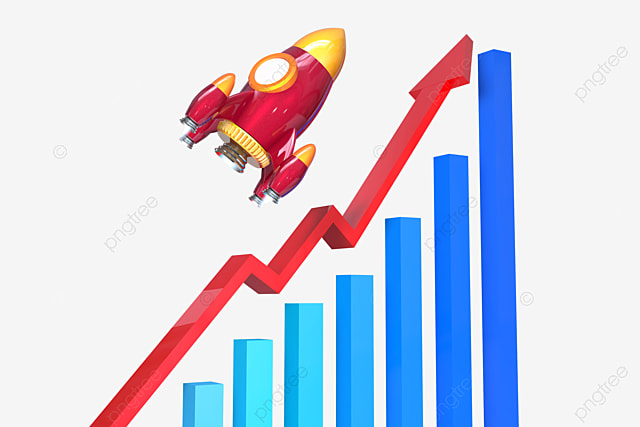
\includegraphics[width=0.8\textwidth]{imgs/curva_rendimiento.jpg} 
    
    \caption{Curva de eficiencia y rendimiento del sistema propuesto.}
    \label{fig:grafico_resultados}
\end{figure}

La curva de rendimiento confirma que el sistema mantiene una eficiencia superior al 95\% incluso bajo condiciones de alta carga.

\lipsum[25]

\section{Modelo de Evaluación}

Para la evaluación final del sistema, se utiliza una métrica combinada $E$ que integra la precisión $P$ y la latencia $L$ de la siguiente manera:

% -------------------------------------------------------------
% ECUACIÓN DE EJEMPLO (Usando el entorno 'equation' para numeración)
% -------------------------------------------------------------
\begin{equation}
    E = \alpha \cdot \frac{P}{100} - \beta \cdot L + \sum_{i=1}^{N} \gamma_i
    \label{eq:evaluacion_final}
\end{equation}

Donde $\alpha$, $\beta$, y $\gamma_i$ son los coeficientes de ponderación, y $N$ es el número total de factores de ruido ambiental. Como se puede observar en la Ecuación (\ref{eq:evaluacion_final}), la precisión contribuye positivamente al valor de $E$, mientras que la latencia la penaliza.
% Nota: La UNEFA Anzoátegui tiene el Capítulo IV como "Análisis e Interpretación de Resultados" [cite: 117]
% --- CAPÍTULO V: CONCLUSIONES Y RECOMENDACIONES ---
\chapter{Conclusiones y Recomendaciones}
\chaptermark{Capítulo V: Conclusiones}
\section{Conclusiones}
\lipsum[25]
\section{Recomendaciones}
\lipsum[26]
\section{Propuesta (si aplica)}
\lipsum[27]
 
% Nota: La UNEFA Anzoátegui tiene el Capítulo V como "Conclusión y Recomendación" [cite: 119]

% =================================================================
% 3. MATERIALES DE REFERENCIA (\backmatter)
% =================================================================
\backmatter

% Referencias
\printbibliography[heading=bibintoc, title={REFERENCIAS BIBLIOGRÁFICAS}] % Se usa el título completo
\cleardoublepage

% Anexos y Apéndices (Se cargan desde el archivo de enlace)
% =================================================================
% ARCHIVO DE ENLACE: ANEXOS Y APÉNDICES (anexos/lista_anexos.tex)
% Contiene la estructura \chapter* y la llamada a los archivos de contenido.
% =================================================================

% --- ANEXOS ---
% Los anexos suelen ser materiales creados por otros o datos brutos (fotos, permisos).
\chapterToc{ANEXOS}
%\cleardoublepage % Agregar si se quiere una página nueva

% Cargar los archivos de contenido de Anexos
\section*{ANEXO A: Memoria Fotográfica de la Aplicación de Instrumentos}
\addcontentsline{toc}{section}{ANEXO A: Memoria Fotográfica de la Aplicación de Instrumentos}

El presente anexo incluye las evidencias fotográficas que demuestran la aplicación de los instrumentos de recolección de datos y el proceso de observación en el sitio de estudio. Se garantiza la anonimidad de los participantes, ocultando sus rostros en las imágenes.

% Aquí se incluirían las figuras de las fotos. Ejemplo:
% \begin{figure}[h]
%     \centering
%     \includegraphics[width=0.8\textwidth]{imgs/foto_entrevista.jpg}
%     \caption{Aplicación del cuestionario a la muestra.}
% \end{figure}

\lipsum[30-31] % ANEXO A: Memoria Fotográfica
\cleardoublepage

% Si tienes un Anexo B, lo añades aquí
% \input{anexos/anexo_b.tex} % ANEXO B: Datos estadísticos brutos
% \cleardoublepage

% ... y así sucesivamente...


% --- APÉNDICES ---
% Los apéndices suelen ser materiales creados por el autor (cuestionarios, códigos, teoría, validaciones).
\chapterToc{APÉNDICES}
%\cleardoublepage % Agregar si se quiere una página nueva

% Cargar los archivos de contenido de Apéndices
\sectionToc{APÉNDICE A: Constancia de Validación y Juicio de Expertos}

Este apéndice contiene la documentación de soporte técnico para el instrumento de recolección de datos. Se incluye la Matriz de Juicio de Expertos y las constancias de validación emitidas por los tres (3) profesionales especializados en el área de Metodología e Ingeniería, tal como lo exige el Manual de Normas \textcite{online:unefa2022}.

\lipsum[32]

\subsection*{Matriz de Consistencia y Validación}
La matriz resume las observaciones y la puntuación de los ítems del instrumento, confirmando su validez de contenido y constructo.

\lipsum[33-34] % APÉNDICE A: Constancia de Validación
\cleardoublepage

% Si tienes un Apéndice B (ej. listado de código), lo añades aquí
% \input{codigo/listado_a.tex} % APÉNDICE B: Listado de Código Fuente
% \cleardoublepage

% ... y así sucesivamente...

\end{document}
